\newcommand\PATH{/home/quentin/informatique-mp2i/02-codage-des-nombres.latex}

\RequirePackage{fix-cm}
\documentclass{scrartcl}

% Fichier pour les dépendances

% Fontes Computer Modern
\usepackage{lmodern}

% Minted
\usepackage[cache=true,outputdir=\PATH/obj]{minted}

% Pour les symboles et outils mathématiques
\usepackage{amsmath}
\usepackage{amsfonts}
\usepackage{amssymb}
\usepackage{mathtools}
\usepackage{cancel}
\usepackage{mathrsfs}
\usepackage{stmaryrd}

% Pour les dessins / images
\usepackage{xcolor}
\usepackage{tikz}
\usepackage{graphicx}

% Tableaux et listes
\usepackage{tabularx}
\newcolumntype{Y}{>{\centering\arraybackslash}X}
\usepackage{booktabs}
\usepackage{multirow}
\usepackage{enumitem}
\usepackage{multicol}
\usepackage{adjustbox}

% Présentation de la page (bordures)
\usepackage[a4paper,top=1cm,bottom=1cm,includefoot,left=1.5cm,right=1.5cm,footskip=1cm]{geometry}
\usepackage{scrlayer-scrpage}
\rofoot*{\pagemark}
\cofoot*{}
\pagestyle{scrheadings}

% Autres
\usepackage{ulem} % Soulignage
\usepackage[french]{babel} % Babel, pour respecter les standards français
\frenchbsetup{StandardLists=true} % ... sauf pour les immondes listes à tirets
\usepackage[T1]{fontenc}

\usepackage{hyperref} % Pour les liens
\hypersetup{
    colorlinks=true,
    linkcolor=blue,
    filecolor=magenta,
    urlcolor=cyan,
}


%% Commandes personnalisées

% Code
\newenvironment{code}[1]
{\VerbatimEnvironment\begin{minted}[breaklines,frame=single,autogobble,linenos,bgcolor=codebg,tabsize=4,mathescape=true]{#1}}
{\end{minted}}
\definecolor{codebg}{gray}{1}
\newenvironment{algotext}
{\VerbatimEnvironment\begin{minted}[frame=single,autogobble,linenos,bgcolor=codebg,tabsize=4,escapeinside=||,mathescape=true]{text}}
{\end{minted}}


% Paragraphes spéciaux
\newcounter{compteurExos}
\setcounter{compteurExos}{0}
\newcommand{\plabel}[1]{{\parindent10pt \fontfamily{cmss}\selectfont\textbf{#1} \,}}

\newcommand{\prop}[1]{\plabel{Propriété :} \textsl{#1}}
\newcommand{\lemma}[1]{\plabel{Lemme :} \textsl{#1}}
\newcommand{\rem}{\plabel{Remarque :}}
\newcommand{\exemple}{\plabel{Exemple :}}
\newcommand{\exo}{\stepcounter{compteurExos}\plabel{Exercice \thecompteurExos :}}
\newcommand{\obs}{\plabel{Observation :} }

\newenvironment{demo}{\begin{itemize}[label=$\triangleright$]}{\end{itemize}}
\newcommand{\definition}{\parindent0pt }
\newcommand{\semidef}{\parindent0pt $\bullet$ \,}

% Outils
\newcommand{\corrpar}{\vspace{-20pt}}
\newcommand{\extraspace}{\vspace{5pt}}

% Configuration
\parskip5pt

% Annonce pour le développement:
\newcommand{\notecentrale}[1]{\begin{center}\textsl{#1}\end{center}}
\newcommand{\warnwip}{\notecentrale{Ce cours n'est pas encore bien relu}}
\newcommand{\warnwipnext}{\notecentrale{La suite de ce cours est encore en rédaction}\message}


\newcommand{\set}[1]{{\{#1\}}}
\newcommand{\intset}[1]{\llbracket #1 \rrbracket}
\newcommand{\intsete}[1]{\llbracket #1 \llbracket}
\newcommand{\inteset}[1]{\rrbracket #1 \rrbracket}
\newcommand{\intesete}[1]{\rrbracket #1 \llbracket}

\newcommand{\tq}{\, \big| \,}

\newcommand{\card}{\.\textmd{card}}
\newcommand{\Id}{\textsl{Id}}
\newcommand{\supp}{\text{supp}}

% Partie entière, arrondi supérieur

\DeclarePairedDelimiter\ceil{\lceil}{\rceil}
\DeclarePairedDelimiter\floor{\lfloor}{\rfloor}



\newcommand{\fpq}{\mathbb{F}_p(Q)}
\newcommand{\abins}{\mathscr{A}_B(\mathcal{S})}
\newcommand{\pb}[3]
{
	\textbf{#1}
	\left|\left|\begin{tabular}{l l}
		Entrée: & #2 \\
		\vspace{-10pt} & \\
		\hline
		\vspace{-10pt} & \\
		Sortie: & #3
	\end{tabular}\right.\right.
}
\newcommand{\pbinlist}[3]
{
	\textbf{#1} &  $\left|\left|\begin{tabular}{l l}
		Entrée: & #2\\ 
		\vspace{-10pt} & \\
		\hline
		\vspace{-10pt} & \\
		Sortie: & #3 
	\end{tabular}\right.\right.$ 
}
\newcommand{\val}{\text{val}}
\newcommand{\argmax}{\mathop{\text{argmax}}}
\newcommand{\argmin}{\mathop{\text{argmin}}}

\setlength{\parindent}{0pt}

\title{Codage des nombres}
\author{}
\date{}

\begin{document}
	\maketitle
	\section{Codage des entiers naturels}

	Soit $b \in \mathbb{N} \setminus \{0,1\}$.
	On note $\Sigma = [0..b-1]$.
	Les éléments de $\Sigma$ seront appelés les chiffres et les mots sur $\Sigma$ seront appelés des nombres.

		\subsection{Codage en base b}

			\subsubsection{Définition}
					
				$val_b = \left( \begin{array}{ccc} \Sigma^* & \to & \mathbb{N} \\ 
				a_{l-1}a_{l-2}...a_0 & \mapsto & \displaystyle \sum_{i=0}^{l-1} a_ib^i \end{array} \right)$
				où $\displaystyle \Sigma^* = \bigcup_{i \in \mathbb{N}} \Sigma^i$, 
				c'est-à-dire l'ensemble des suites de longueur $i$ dans $\Sigma$ pour $i \in \mathbb{N}$.

				\noindent \rem le mot vide sera noté $\varepsilon$ $(\Sigma^0 = \{\varepsilon\})$ et on a $val_b(\varepsilon) = 0$.
				
				\noindent \exemple 
					$val_{10}(123) = 1 \times 10^2 + 2 \times 10^1 + 3 \times 10^0 = 100 + 20 + 3 = 123$
					
					$val_2(100) = 1 \times 2^2 + 0 \times 2^1 + 0 \times 2^0$

			\subsubsection{Taille du codage}
				
				\noindent \lemma Soit $l \in \mathbb{N}$. $\forall a \in \Sigma^l$, $val_b(a) \in [0..b^l[$.
				\begin{demo}
					\item 
						Soit $(a_{l-1},a_{l-2},...,a_0) \in \Sigma^l$. \newline
						$val_b(a_{l-1}a_{l-2}...a_0) = \sum_{i=0}^{l-1} a_ib^i$.
						Or $\forall i \in [0..l-1], a_i \leqslant (b-1)$.
						
						Donc $\displaystyle val_b(a_{l-1}a_{l-2}...a_0) \leqslant \sum_{i=0}^{l-1} (b-1)b^i
						= \sum_{i=0}^{l-1} b^{i+1} - \sum_{i=0}^{l-1} b^i 
						= \sum_{i=1}^l b^i - \sum_{i=0}^{l-1} b^i 
						= b^l - b^0 
						= b^l - 1$
				\end{demo}

				\noindent \prop Soit $n \in \mathbb{N}$. \newline
				Il faut $\lceil log_b(n+1) \rceil$ chiffres au minimum pour écrire $n$ en base $b$.

				\begin{demo}
					\item
						On note $l = \lceil log_b(n+1) \rceil$.

						Par l'absurde, supposons que $a_{l-1}...a_0 \in \Sigma^{l'}$ représente $n$ en base $b$ avec $l' < l$ chiffres.

						On a $l' < log_b(n+1)$ par définition de la partie entière supérieure comme plus petit majorant entier.

						$n = val_b(a_{l'-1}a_{l'-2}...a_0) \leqslant b^{l'}-1 < n+1$.
						Or $b^{l'} < b^{log_b(n+1)} = n+1$.
						Donc $n < n+1-1 \iff n < n$. ABSURDE.
				\end{demo}

			\subsubsection{Existence}

				\noindent \rem Pour tout $n \in \mathbb{N}$, il existe $a_{l-1}a_{l-2}...a_0 \in \Sigma^l$ tel que
				$val_b(a_{l-1}...a_0) = n$. Plus précisément, tout entier $n \in \mathbb{N}$ admet une écriture en base $b$
				à $\lceil lob_b(n+1) \rceil$ chiffres.

				\begin{demo}
					\item
						Montrons par récurrence sur $l \in \mathbb{N}$ la propriété $\mathcal{P}_l$ :
						"$\forall n \in [0..b^l-1], n$ admet une écriture en base $b$ à $l$ chiffres".

						$\forall n \in [0..b^l-1]$, c'est-à-dire $\forall n \in [0..0], n$ admet une écriture en base $b$ à $0$ chiffres.
						En effet, le seul nombre à $0$ chiffre est le mot vide $\varepsilon$.
						Par convention, $val_b(\varepsilon) = 0 \in [0..0]$.
						Donc $\mathcal{P}_0$ est vraie.

						Pour un $l$ fixé, supposons $\mathcal{P}_l$. Soit $n \in [0..b^{l+1}-1[$.
						Par définition de la division euclidienne, il existe $(q,r) \in \mathbb{N}^2$ tel que
						$n = b^lq+r$ et $r < b^l$, $i.e.$ $r \in [0..b^l-1[$.
						Par $\mathcal{P}_l$, on en déduit que $r$ admet une écriture en base $b$ à $l$ chiffres qu'on note $(a_i)_{i \in [0..l[}$.
						On a alors $r = \sum_{i=0}^{l-1} a_ib^i$, et donc $n=qb^l + \sum_{i=0}^{l-1} a_ib^i$.

						Puisque $n < b^{l+1}$, on a nécessairement $q < b$ (sinon on aurait $n \geqslant qb^l > b \times b^l = b^{l+1}$).
						Ainsi, en posant $a_l = q$, on a $(a_i)_{i \in [0..l+1[} \in \Sigma^{l+1}$ et $n = a_lb^l + \sum_{i=0}^{l-1} a_ib^i$.

						Donc $n$ admet bien une écriture en base $b$ à $l+1$ chiffres. Donc $\mathcal{P}_{l+1}$ est vraie.
				\end{demo}

			\subsubsection{Quasi-unicité}
				
				\noindent \prop Soit $n \in \mathbb{N}$.
				Si $a_{l-1}a_{l-2}...a_0 \in \Sigma^l$ est une écriture de $n$ en base $b$ (c'est-à-dire si $val_b(a_{l-1}...a_0) = n$)
				alors $\forall k \in [0..l-1], a_k$ est le reste modulo $b$ du quotient de $n$ par $b^k$.

				\noindent \exemple $b=10, n=123, a_2=1, a_1=2=(n//10)\%10, a_0=3=n\%10$

				\begin{demo}
					\item
						Soit $n \in \mathbb{N}$, soit $a_{l-1}...a_0$ une écriture de $n$ en base $b$. Soit $k \in [0..l-1]$.
						On a : $$n = val_b(a_{l-1}...a_0) = \sum_{i=0}^{l-1} a_ib^i = 
						\sum_{i=0}^{k-1} a_ib^i + \sum_{i=k}^{l-1} a_ib^i =
						\sum_{i=0}^{k-1} a_ib^i + \sum_{i=k}^{l-1} a_i(b^k \times b^{i-k}) =
						\underbrace{\sum_{i=0}^{k-1} a_ib^i}_{=r_k} + b^k \underbrace{\sum_{i=k}^{l-1} b^{i-l}}_{=q_k}$$

						On note $r_k = \sum_{i=0}^{k-1} a_ib^i$. On a $r_k \in \mathbb{N}$ et puisque $\forall i \in [0..l[, a_i \in [0..b[$, on a aussi :
						$$r_k \leqslant \sum_{i=0}^{k-1} (b-1)b^i = \sum_{i=0}^{k-1} b^{i+1} - \sum_{i=0}^{k-1} b^i = b^k-1 < b^k$$.

						On note $q_k = \sum_{i=0}^{k-1} a_ib^{i-k}$. Puisque $i-k \geqslant 0 \forall i \in [k..l[$, alors $b^{i-k} \in \mathbb{N}$,
						ainsi $q_k$ est une somme d'entiers positifs donc $q_k \in \mathbb{N}$.
						On en déduit de la première égalité que $q_k$ est le quotient et $r_k$ le reste dans la division euclidienne de $n$ par $b^k$.
						On cherche donc à montrer que $a_k$ est le reste modulo $b$ de $q_k$. On a :
						$$q_k = \sum_{i=k}^{l-1} a_ib^{i-k} = a_k\underbrace{b^{k-k}}_{=1} + \sum_{i=k+1}^{l-1} a_i(b^{i-k-1} \times b)
						= a_k + b \left( \sum_{i=k+1}^{l-1} a_ib^{i-k-1} \right)$$

						D'une part on sait que $a_k < b$ car $a_k \in \Sigma$. D'autre part, comme $i-k-1 \geqslant 0 \forall i \in [k+1..l-1],
						\sum_{i=k+1}^{l-1} a_ib^{i-k-1} \in \mathbb{N}$. On en déduit donc de l'égalité précédente que $a_k$ est bien le reste de $q_k$ modulo $b$.
				\end{demo}

			\subsubsection{Conclusion}

				Pour $l \in \mathbb{N}$, on note $ec_b^l$ la fonction qui à un entier de $[0..b^l[$ associe son écriture en base $b$ à $l$ chiffres.

		\subsection{Addition en base 2}

			\begin{figure}[H]
				\centering
				\fbox{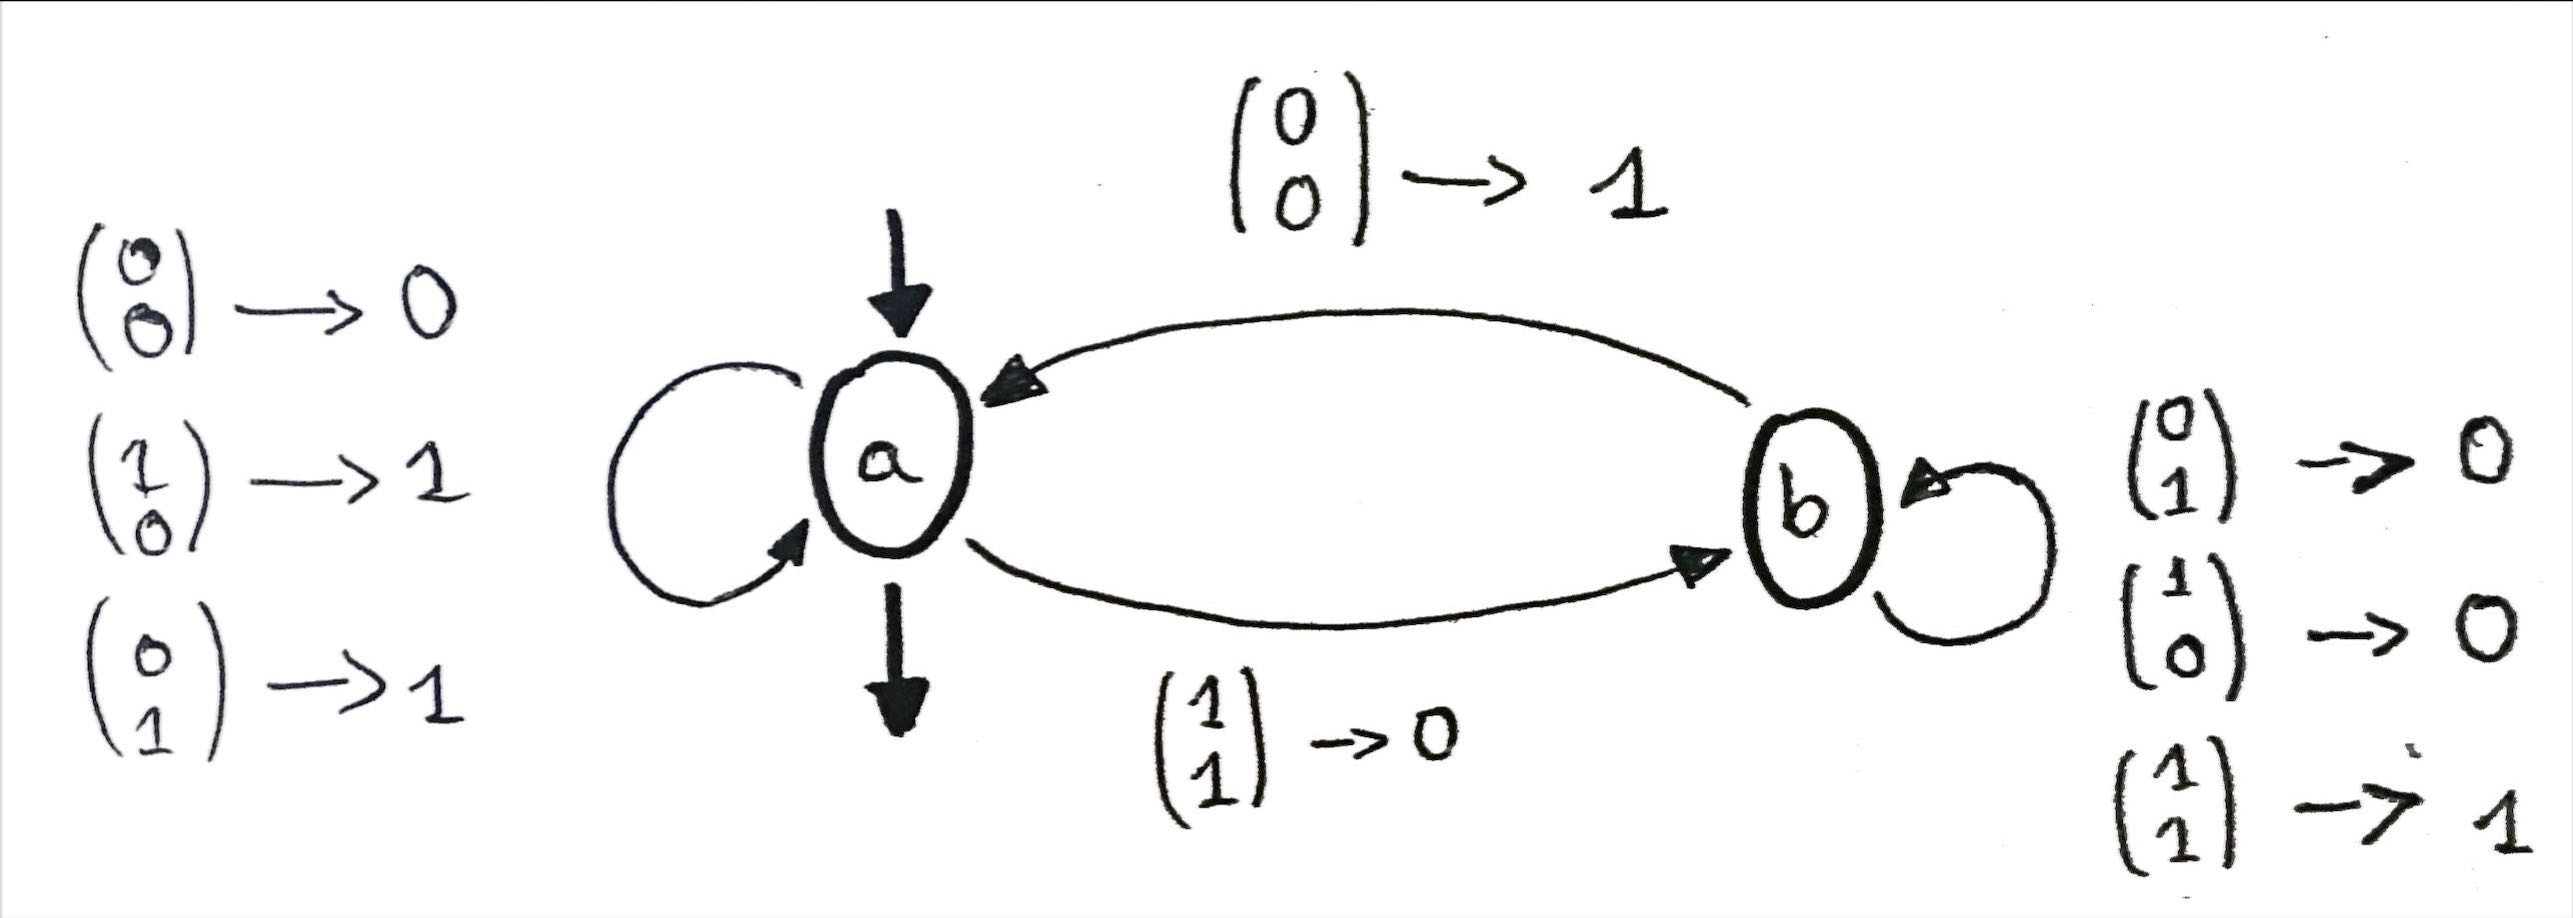
\includegraphics[width = 0.5\textwidth]{addition_base_2.jpeg}}
				\caption{Addition en base 2}
				\hfill
			\end{figure}

		\subsection{Application}

			Pour $u \in \mathbb{N}^{\mathbb{N}}$, on note
			\[
				\pb{$\mathcal{P}_u$}{$n \in \mathbb{N}$}{$u_n$}
			\]
			$\underbrace{A}_{\texttt{un algo}} \iff \texttt{suite finie de caractère} 
			\iff \texttt{suite finie d'entiers entre 0 et 255}$

			$\iff \texttt{un entier écrit en base 256}$.

			On note $\varphi$ la fonction qui a un algorithme $A$ associe un entier écrit en base $256$ 
			en remplaçant les caractères de l'algorithme pour un entier entre $1$ et $255$.

			\[
			\varphi = \left( \begin{array}{ccc}
			\textrm{l'ensemble des textes des algorithmes} & \to & \mathbb{N} \\
			n \in \mathbb{N} & \mapsto & p \\
			\end{array} \right)
			\]

			$\varphi$ est injective mais pas surjective. $\varphi \Big|_{A}^{Im(\varphi)}$ est bijective.

			On note pour $A$ le texte d'un algo qui prend en entrée un entier et qui rend en sortie un entier, $eval(A,n)$, la valeur
			absolue en lançant cet algorithme sur l'entrée $n$.

			\rem Si $A$ résout $\mathcal{P}_n$ pour $u \in \mathbb{N}^{\mathbb{N}}$, alors $\forall n \in \mathbb{N}$, 
			$eval(A,n) = u_n$.


			On définit $u \in \mathbb{N}^{\mathbb{N}}, u_n = \left\{ 
			\begin{array}{ll} eval(\varphi^{-1}(n),n)+1 & \mbox{si } n \in Im(\varphi) \\
			0 & \mbox{sinon} \\
			\end{array} \right. $


			On suppose que $A$ est un algorithme qui résout le problème $\mathcal{P}_u$. Alors :
			\begin{align*}
				eval(A_u, \varphi(A_u)) &= u_{\varphi(A_u)} \mbox{	car } A \mbox{ résout } \mathcal{P}_u \\
				&= eval(\varphi^{-1} (\varphi(A_u)), \varphi(A_u)+1) \\
				&= eval(A_u, \varphi(A_u)) +1 \\
			\end{align*}
			ABSURDE. Donc il n'existe pas d'algorithme résolvant $\mathcal{P}_u$.

			\underline{Notation de l'addition en base 2 :}

			Pour $l \in \mathbb{N}$ et $\Sigma = \{0,1\}$,
				


\end{document}
